\documentclass[border=3pt]{standalone}
\usepackage{tikz}
\usetikzlibrary{calc}
\begin{document}
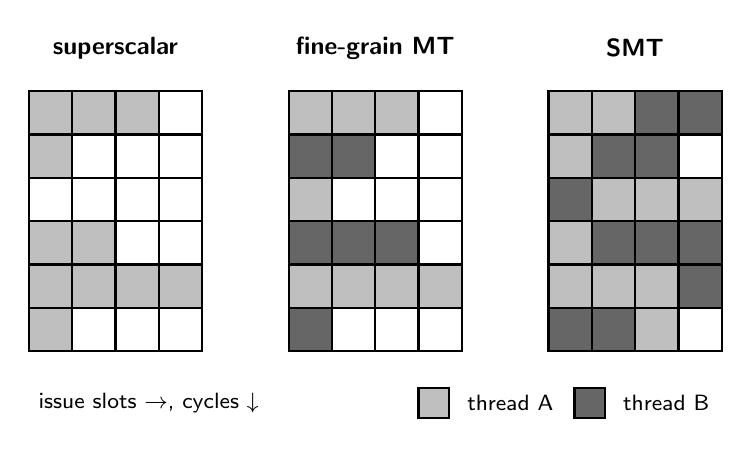
\begin{tikzpicture}[font=\sffamily\small, x=5.5mm, y=5.5mm]
  % thread A = black!25, thread B = black!60, 0 = empty
  % superscalar: one thread, wasted slots
  \begin{scope}[shift={(0,0)}]
    \node[font=\sffamily\small\bfseries] at (2,7.0) {superscalar};
    \foreach \r/\pattern in {5/{25,25,25,0}, 4/{25,0,0,0}, 3/{0,0,0,0}, 2/{25,25,0,0}, 1/{25,25,25,25}, 0/{25,0,0,0}}{
      \foreach [count=\c] \v in \pattern {
        \ifnum\v=0 \draw[thick] (\c-1,\r) rectangle (\c,\r+1);
        \else \draw[thick, fill=black!\v] (\c-1,\r) rectangle (\c,\r+1); \fi}}
  \end{scope}
  % fine-grain MT: rows alternate threads
  \begin{scope}[shift={(6,0)}]
    \node[font=\sffamily\small\bfseries] at (2,7.0) {fine-grain MT};
    \foreach \r/\pattern in {5/{25,25,25,0}, 4/{60,60,0,0}, 3/{25,0,0,0}, 2/{60,60,60,0}, 1/{25,25,25,25}, 0/{60,0,0,0}}{
      \foreach [count=\c] \v in \pattern {
        \ifnum\v=0 \draw[thick] (\c-1,\r) rectangle (\c,\r+1);
        \else \draw[thick, fill=black!\v] (\c-1,\r) rectangle (\c,\r+1); \fi}}
  \end{scope}
  % SMT: threads mixed within a cycle
  \begin{scope}[shift={(12,0)}]
    \node[font=\sffamily\small\bfseries] at (2,7.0) {SMT};
    \foreach \r/\pattern in {5/{25,25,60,60}, 4/{25,60,60,0}, 3/{60,25,25,25}, 2/{25,60,60,60}, 1/{25,25,25,60}, 0/{60,60,25,0}}{
      \foreach [count=\c] \v in \pattern {
        \ifnum\v=0 \draw[thick] (\c-1,\r) rectangle (\c,\r+1);
        \else \draw[thick, fill=black!\v] (\c-1,\r) rectangle (\c,\r+1); \fi}}
  \end{scope}
  % legend and axes
  \node[anchor=west, font=\sffamily\footnotesize] at (0,-1.2) {issue slots $\rightarrow$, cycles $\downarrow$};
  \draw[thick, fill=black!25] (9.0,-1.55) rectangle +(0.7,0.7); \node[anchor=west, font=\sffamily\footnotesize] at (9.9,-1.2) {thread A};
  \draw[thick, fill=black!60] (12.6,-1.55) rectangle +(0.7,0.7); \node[anchor=west, font=\sffamily\footnotesize] at (13.5,-1.2) {thread B};
\end{tikzpicture}
\end{document}
